\graphicspath{{3series/asy/}}

\thispagestyle{empty}

\setcounter{section}{2}
\section{Series}\label{chap:series}

\setcounter{subsection}{13}
\subsection{Infinite Series and the Series Tests}\label{sec:series}

For millennia, certainly since Zeno's paradoxes of c.\,430\,\BC, mathematicians have been interested in the meaning and evaluation of infinite sums such as
\[
	\sum_{n=1}^\infty \frac 1{n^2}=1+\frac 14+\frac 19+\frac 1{16}+\cdots
\]
The standard approach in modern mathematics is to outsource the definition to that of \emph{limits.}

\begin{defn}{}{}
	The \emph{$n\th$ partial sum} $s_n$ of a sequence $(a_n)_{n=m}^\infty$ is the \textbf{finite sum}
	\[
		s_n:=\smash{\sum_{k=m}^n}a_k=a_m+a_{m+1}+\cdots+a_n
	\]
	\begin{itemize}\itemsep2pt
	  \item The \emph{(infinite) series}\footnotemark{} $\smash[b]{\sum\limits_{n=m}^\infty a_n}$ is the limit $\lim s_n$ of the sequence $(s_n)$ of partial sums.
	  \item A series \emph{converges, s to $\pm\infty$} or \emph{diverges by oscillation} as does the sequence $(s_n)$.
	  \item $\sum a_n$ \emph{converges absolutely} if $\sum\nm{a_n}$ converges.
	  \item $\sum a_n$ \emph{converges conditionally} if it converges but not absolutely ($\sum \nm{a_n}$ diverges to $\infty$).
	\end{itemize}
\end{defn}

\footnotetext{%
	If the initial term is understood or is irrelevant to the situation, it is common to write $\sum a_n$.%
}

We don't (yet) know whether our motivating example converges, but at least we have a meaning:
\[
	\sum_{n=1}^\infty \frac 1{n^2}
	=\lim s_n\quad\text{where}\quad s_n=\sum\limits_{k=1}^n \frac 1{k^2}=1+\frac 14+\cdots+\frac 1{n^2}
\]

\begin{thm}{Basic Series Laws}{basicserieslaws}
	Infinite series behave nicely with respect to addition and scalar multiplication. For instance:
	\begin{enumerate}\itemsep2pt
	  \item If $\sum a_n$ is convergent and $k$ is constant, then $\sum ka_n=k\sum a_n$ is convergent.
	  \item If $\sum a_n$ and $\sum b_n$ are convergent, then $\sum(a_n\pm b_n)=\sum a_n\pm\sum b_n$ are also convergent.
	  \item If $\sum a_n=\infty$ and $k>0$, then $\sum ka_n=\infty$.
	  \item If $\sum a_n=\infty$ and $\sum b_n$ converges, then $\sum(a_n+b_n)=\infty$.
	\end{enumerate}
\end{thm}

\begin{proof}
	Simply apply the limit/divergence laws to the sequence of partial sums. E.g.{} for 1,
	\[
	  \sum ka_n = \lim_{n\to\infty}\sum_{j=m}^nka_j \overset{\text{finite}}{\overset{\text{sum}}{=}} 
	  \lim_{n\to\infty}k\sum_{j=m}^na_j \overset{\text{limit}}{\overset{\text{laws}}{=}}
	  k\lim_{n\to\infty}\sum_{j=m}^na_j =k\sum a_n
	\]
	The others may be proved similarly.
\end{proof}


Series \textbf{do not} behave nicely with respect to multiplication (see also Exercise \ref{exs:seriesmult}):
\[
	a_1b_1+a_2b_2+\cdots 
	=\sum a_nb_n\neq \bigl(\sum a_n\bigr)\bigl(\sum b_n\bigr) 
	=\bigl(a_1+a_2+\cdots\bigr)\bigl(b_1+b_2+\cdots\bigr)
\]

\goodbreak


\boldsubsection{Series which may be evaluated exactly}

Given a series $\sum a_n$, our primary goal is to answer a simple question: ``Does it converge?'' Even when the answer is \emph{yes,} a precise computation of the limit will usually be beyond us. We instead develop techniques (the upcoming \emph{series tests}) which typically rely on comparing $\sum a_n$ to some `standard' series whose properties are completely understood: in particular\ldots

\begin{defn}{Geometric series}{}
	A sequence $(a_n)$ is \emph{geometric} if the ratio of successive terms is constant: $a_n=ba^n$ for some constants $a,b$. A \emph{geometric series} is the sum of a geometric sequence. 
\end{defn}

The computation of the sequence of partial sums should be familiar (for simplicity assume $b=1$)
\[
	(1-a)s_n
	=\bigl(a^m+\textcolor{blue}{a^{m+1}+\cdots+a^n}\bigr)
	-\bigl(\textcolor{blue}{a^{m+1}+a^{m+2}+\cdots +a^n}+a^{n+1}\bigr) 
	=a^m-a^{n+1}
\]
from which we quickly conclude:

\begin{thm}{}{geomseries}
	Suppose $a$ is constant. Then
	\[
		s_n=\sum_{k=m}^n a^k=
		\begin{cases}
			\dfrac{a^m-a^{n+1}}{1-a}&\text{if }a\neq 1\\
			n+1-m&\text{if }a=1
		\end{cases}
		\implies \sum_{n=m}^\infty a^n
		\begin{cases}
			\text{converges to }\dfrac{a^m}{1-a}&\text{if }\nm{a}<1\\
			\text{diverges to $\infty$}&\text{if }a\ge 1\\
			\text{diverges by oscillation}&\text{if }a\le -1
		\end{cases}
	\]
	In particular, $\sum a^n$ converges absolutely if $\nm a<1$ and diverges otherwise. 
\end{thm}


\begin{examples}{}{}
	\exstart $\displaystyle \sum_{n=-1}^\infty 2\left(-\frac 45\right)^n
		=2\frac{\left(-\frac 45\right)^{-1}}{1+\frac 45} 
		=-\frac 52\cdot\frac 59
		=-\frac{25}{18}$
	\begin{enumerate}\setcounter{enumi}{1}
	  \item Consider the series $\sum a_n=\smash[b]{\sum\limits_{n=3}^\infty} \left(\frac 25\right)^n +2^n$. If this were convergent, then
		\[
			\sum 2^n=\sum a_n-\sum\left(\frac 25\right)^n
		\]
		would converge (Theorem \ref{thm:basicserieslaws}); a contradiction.
	\end{enumerate}
\end{examples}


\boldinline{Telescoping series}

A rarer type of series can be evaluated using the algebra of partial fractions.

\begin{example}{}{}
	To compute $\sum\limits_{n=1}^\infty\frac 1{n(n+1)}$, first  observe that
	\[
		s_n=\sum_{k=1}^n\frac 1{k(k+1)} 
		=\sum_{k=1}^n\frac 1k-\frac 1{k+1} 
		=\frac 11\textcolor{blue}{-\frac 12+\frac 12-\frac 13+\cdots+\frac 1n}-\frac 1{n+1}
		=1-\frac 1{n+1}
	\]
	It follows that
	\[
		\sum_{n=1}^\infty\frac 1{n(n+1)}
		=\lim \left(1-\frac 1{n+1}\right)=1
	\]
	Similar arguments can be made for other series such as $\sum\frac 1{n(n+2)}$.
\end{example}


\goodbreak


\boldsubsection{The Cauchy Criterion}

The starting point for our general series tests uses Cauchy completeness.

\begin{example}{}{convserieseuler}
	Consider again the series $\sum\frac 1{n^2}$. We show that the sequence of partial sums $(s_n)$ is Cauchy. Suppose $\epsilon>0$ is given and let $N=\frac 1\epsilon$. Then,
	\begin{align*}
		m>n>N\implies \nm{s_m-s_n}
		&=\sum_{k=n+1}^m\frac 1{k^2}<\sum_{k=n+1}^m\frac 1{k(k-1)} 
		=\sum_{k=n+1}^m\frac 1{k-1}-\frac 1k\\
		&=\frac 1n-\frac 1m<\frac 1N =\epsilon
	\end{align*}
	where most terms cancel analogous to the telescoping series approach. By Cauchy completeness (Theorem \ref{thm:convcauchy}), $(s_n)$ converges and we conclude
	\[
		\tcbhighmath{\sum\frac 1{n^2}\ \text{ converges}}
	\]
	Computing the value of this series is significantly harder: a sketch argument for why $\sum_{n=1}^\infty\frac 1{n^2}=\frac{\pi^2}6$ is in Exercise \ref{exs:eulersum}.
\end{example}

\begin{thm}{Cauchy criterion for series}{}
	A series $\sum a_n$ converges precisely when
	\[
		\forall\epsilon>0,\ \exists N\text{ such that }m> n>N
		\implies\nm{s_m-s_{n}}=\nm{\sum_{k=n+1}^ma_k}<\epsilon
	\]
\end{thm}

The previous example essentially verified the Cauchy criterion for $\sum\frac 1{n^2}$.

\begin{proof}
	Let $(s_n)$ be the sequence of partial sums. Then
	\begin{align*}
		\sum a_n\text{ converges}
		&\iff (s_n)\text{ converges}\\
		&\iff (s_n)\text{ is a Cauchy sequence} 
		\tag{Theorem \ref{thm:convcauchy}}\\
		&\iff \Bigl(\forall\epsilon>0,\ \exists N\text{ such that }m> n>N
		\Longrightarrow\nm{s_m-s_n}<\epsilon\Bigr)
		\tag*{\qedhere}
	\end{align*}
\end{proof}

\begin{example}{}{harmonic}
	For contradiction, suppose that the \emph{harmonic series} $\sum\frac 1n$ converges. Take $\epsilon=\frac 12$ in the Cauchy criterion to observe that
	\[
		\exists N\text{ such that }m> n>N\implies \nm{\sum_{k=n+1}^{m}\frac 1k}<\frac 12
	\]
	However, taking $m=2n$ (plainly $m>n$ since $n>N\ge 1$) results in a contradiction: 
	\[
		\frac 12>\nm{\sum_{k=n+1}^{m}\frac 1k}=\nm{\frac 1{n+1}+\cdots+\frac 1m}\ge \frac{m-n}{m}=1-\frac nm=\frac 12
	\]
	We conclude that the harmonic series diverges to $\infty$.
\end{example}

\goodbreak


\boldsubsubsection{The Series Tests}

For the remainder of this section we develop tests for the convergence/divergence of an infinite series: the $n\th$-term, comparison, root and ratio tests. The first follows quickly from the Cauchy criterion.

\begin{thm}{Divergence/$n\th$-term test}{}
	If $\lim a_n\neq 0$ then $\sum a_n$ is divergent.
\end{thm}

\begin{proof}
	We prove the contrapositive. Suppose $\sum a_n$ is convergent, and that $\epsilon>0$ is given. Take $m=n+1$ in the Cauchy criterion. Then
	\[
		\exists \tilde N \text{ such that }m>\tilde N\implies\nm{a_{m}}<\epsilon \tag{let $\tilde N=N+1$}
	\]
	Otherwise said, $\lim a_n=0$.
\end{proof}


\begin{examples}{}{}
	\exstart The series $\sum\sin(\frac{n\pi}9)$ diverges.
	\begin{enumerate}\setcounter{enumi}{1} 
	  \item The $n\th$-term test tells us that the geometric series $\sum a^n$ diverges whenever $\nm a\ge 1$. We still need our earlier analysis (Theorem \ref{thm:geomseries}) for when $\nm a<1$.
	  \item The \textbf{converse} of the $n\th$-term test is \textbf{false!} Example \ref{ex:harmonic} provides the canonical example: the \textbf{divergent} harmonic series $\sum \frac 1n$ also satisfies $\lim\frac 1n=0$.
	\end{enumerate}
\end{examples}


\begin{thm}{Comparison test}{}
	\exstart Let $\sum b_n$ be a convergent series of non-negative terms and assume $\nm{a_n}\le b_n$ for all (large) $n$. Then both $\sum a_n$ and $\sum \nm{a_n}$ are convergent.
	\begin{enumerate}\setcounter{enumi}{1}
	  \item If $\sum a_n=\infty$ and $a_n\le b_n$ for all (large) $n$, then $\sum b_n=\infty$.
	\end{enumerate}
\end{thm}

\begin{proof}
	Suppose ``large $n$" means $n>M$ for some fixed $M$. 
	\begin{enumerate}
	  \item Let $\epsilon>0$ be given. Since $\sum b_n$ converges, $\exists N\ge M$ such that
		\[
			m>n>N\implies\nm{\sum_{k=n+1}^ma_k}
			\overset{\triangle}{\le}
			\sum_{k=n+1}^m\nm{a_k}\le\sum_{k=n+1}^mb_k
			<\epsilon
		\]
		\item The $n\th$ partial sum (post $M$) of $\sum b_n$ is
		\[
			\sum_{k=M+1}^nb_k\ge \sum_{k=M+1}^na_k\to \infty \tag*{\qedhere}
		\]
	\end{enumerate}
\end{proof}

\begin{cor}{}{compest}
	\exstart (Absolute convergence implies convergence)\quad Take $\nm{a_n}=b_n$ in part 1 to see that $\sum\nm{a_n}$ convergent $\Longrightarrow\sum a_n$ convergent.
	\begin{enumerate}\setcounter{enumi}{1}
	  \item (Estimation of series)\quad Suppose $\sum b_n$ is a convergent series of non-negative terms and that $\nm{a_n}\le b_n$ for \textbf{all} $n$. Then
	  \[
	  	\sum a_n\le \sum\nm{a_n}\le \sum b_n
	  \]
	\end{enumerate}
\end{cor}

\goodbreak


\begin{examples}{}{compexs}
	\exstart Since the geometric series $\sum \frac 2{3^n}$ converges, $\frac{2n+1}{(n+2)3^n}\le \frac 2{3^n}$, we see that%
	\[
		\sum_{n=0}^\infty\frac{2n+1}{(n+2)3^n}
		\le 2\sum_{n=0}^\infty 3^{-n}
		=\frac 2{1-\frac 13}=3
	\]
	That is, the first series converges (absolutely) to some value $\le 3$.
	
	\begin{enumerate}\setcounter{enumi}{1}
	  \item One can sometimes find a sensible comparison series by considering how $a_n$ behaves for large $n$. For instance, when $n$ is large, $a_n=\smash[b]{\frac{(n^2+1)^{1/2}}{(1+\sqrt n)^4}}$ behaves like $\smash[b]{\frac{n}{n^2}=\frac 1{n}}$. Indeed, when $n\ge 2$,
	  \[
	  	a_n>\frac n{(1+\sqrt n)^4}>\frac n{(2\sqrt n)^4}=\frac 1{16n}
	  \]
	  Comparison with the divergent series $\frac 1{16}\sum \frac 1n$ shows that $\sum a_n$ also diverges to $\infty$.
	  
		\item Since $\ln n<n\implies\frac 1{\ln n}>\frac 1n$, we see that $\sum \frac 1{\ln n}$ diverges to $\infty$ by comparison with $\sum\frac 1n$.
		
	  \item $\sum\frac{\sin n}{n^2}$ converges absolutely by comparison to $\sum\frac 1{n^2}$ (Example \ref{ex:convserieseuler}). Corollary \ref{cor:compest} estimates its value ($\le \frac{\pi^2}6$):
		\begin{gather*}
			\textcolor{red}{\sum_{n=1}^\infty\frac{\sin n}{n^2}} 
			\le \textcolor{blue}{\sum_{n=1}^\infty \frac{\nm{\sin n}}{n^2}} 
			\le \sum_{n=1}^\infty\frac 1{n^2} 
			=\frac{\pi^2}6 
			\tag{approximately $\textcolor{red}{1.014}\le \textcolor{blue}{1.280} \le 1.645$}
		\end{gather*}
		
	  %\item $\sum\frac{(-1)^{n+1}}{n^2}$ converges absolutely by comparison with $\sum\frac 1{n^2}$.
	  
	  
	  \item\label{ex:altharmonic1} The \emph{alternating harmonic series} $s=\sum_{n=1}^\infty\frac{(-1)^{n+1}}n$ converges via a sneaky comparison.\par
	  The series $t=\sum_{n=1}^\infty \frac 1{2n(2n-1)}$ converges by comparison with $\sum\frac 1{4(n-1)^2}$. Its $n\th$ partial sum
	  \[
	  	t_n=\sum_{k=1}^{n}\frac 1{2k(2k-1)}
	  	=\sum_{k=1}^n\left[\frac 1{2k-1}-\frac 1{2k}\right]
	  \]
	  is precisely the \emph{even} partial sum of the alternating harmonic series $s_{2n}=\sum_{k=1}^{2n}\frac{(-1)^{k+1}}k$.\par
	  Plainly $\lim s_{2n}=t$. Moreover $s_{2n+1}=s_{2n}+\frac 1{2n+1}\Longrightarrow \lim s_{2n+1}=t \Longrightarrow \lim s_n=t$. Since the harmonic series $\sum\frac 1n$ diverges (Example \ref{ex:harmonic}), we conclude that the alternating harmonic series \textbf{converges conditionally}. We'll revisit this discussion in the next section.
	  

		\item\label{ex:root5} $\sum\left(\frac n{n+1}\right)^{n^2}$ converges by comparison with $\sum 2^{-n}$. To see this, recall Exercise \ref*{sec:monocauchy}.\ref{exs:edefn}:
		\[
			\left(\frac n{n+1}\right)^n
			=\frac{n+1}n\left(1-\frac 1{n+1}\right)^{n+1}
			\xrightarrow[n\to\infty]{}
			e^{-1}
		\]
		Plainly $e^{-1}<\frac 12$, whence for large $n$,
		\[
			\left(\frac n{n+1}\right)^n\le\frac 12
			\implies 
			\left(\frac n{n+1}\right)^{n^2}\le 2^{-n}
		\]
		In fact $\left(\frac n{n+1}\right)^n$ is monotone-down, whence $e^{-1}\le \left(\frac n{n+1}\right)^n\le \frac 12$ \textbf{for all $n$}, and so
		\[
			0.58198\approx \frac{e^{-1}}{1-e^{-1}}
			=\sum_{n=1}^\infty e^{-n}
			\le \sum_{n=1}^\infty\left(\frac n{n+1}\right)^{n^2}
			\le \sum_{n=1}^\infty 2^{-n}
			=\frac{1/2}{1-1/2}=1
		\]
		A computer estimate yields $\sum\limits_{n=1}^\infty\left(\frac n{n+1}\right)^{n^2}\approx 0.8174$.
	\end{enumerate}
\end{examples}


\goodbreak


Our last two tests in this section are less powerful but often easier to use.


\begin{thm}{Root test}{}
	Suppose $\limsup\nm{a_n}^{1/n}=L$.
	\begin{enumerate}
		\item If $L<1$, then $\sum a_n$ converges absolutely.
		\item If $L>1$, then $\sum a_n$ diverges.
	\end{enumerate}
	If $L=1$, then no conclusion can be drawn.
\end{thm}

We defer the proof until after some examples. By combining with the inequalities of Theorem \ref{thm:rootratio}
	\[
		\liminf\nm{\frac{a_{n+1}}{a_n}}\le\liminf\nm{a_n}^{1/n}\le\limsup\nm{a_n}^{1/n}\le \limsup\nm{\frac{a_{n+1}}{a_n}}
	\]
we obtain a second familiar test.

\begin{cor}{Ratio test}{}
	Suppose $(a_n)$ is a sequence of non-zero terms.
	\begin{enumerate}
		\item If $\smash{\limsup\nm{\frac{a_{n+1}}{a_n}}<1}$, then $\sum a_n$ converges absolutely. 
		\item If $\liminf\nm{\frac{a_{n+1}}{a_n}}>1$, then $\sum a_n$ diverges.
	\end{enumerate}
\end{cor}

In elementary calculus you likely saw the special cases when
\[
	L=\lim\nm{a_n}^{1/n}=\lim\nm{\frac{a_{n+1}}{a_n}}
\]
Our versions are more general since these limits \emph{might not exist.}

\begin{examples}{}{}
\exstart The ratio test is particularly useful for series involving \emph{factorials} and \emph{exponentials.}
\begin{enumerate}\setcounter{enumi}{1}
	\item[]\begin{enumerate}
	  \item $\sum\frac{n^4}{2^n}$ converges, since $\lim\nm{\frac{a_{n+1}}{a_n}}=\lim\frac{(n+1)^4}{2n^4}=\frac 12<1$.
		\item $\sum\frac{n!}{2^n}$ diverges, since $\lim\nm{\frac{a_{n+1}}{a_n}} =\lim\frac{(n+1)!}{2n!}=\lim \frac{n+1}2=\infty$.
	\end{enumerate}
	
	\item Both tests are inconclusive for rational sequences: if $a_n=\frac{b_n}{c_n}$ where $b_n,c_n$ are polynomials, then
	\[
		\lim\nm{\frac{a_{n+1}}{a_n}}=1=\lim\nm{a_n}^{1/n}
	\]
	For example, attempting to apply the ratio test to $\sum\frac{n+5}{n^2}$ results in
	\[
		\lim\nm{\frac{a_{n+1}}{a_n}} =\lim \frac{(n+6)n^2}{(n+5)(n+1)^2}=1
	\]
	This series is divergent by comparison with the harmonic series $\sum \frac 1n$.
	
	
	\item In Example \ref*{ex:compexs}.\ref{ex:root5}, our use of the comparison test was really the root test in disguise:
	\[
		a_n=\left(\frac n{n+1}\right)^{n^2}
		\implies \lim\nm{a_n}^{1/n}
		=\lim\left(\frac n{n+1}\right)^{n}
		=e^{-1}<1 
		\implies \sum a_n\text{ converges}
	\]
	In this case the root test was much easier to apply.
	
	
	\goodbreak
	
	
	\item The ratio test is the weakest test thus far; certainly it does not apply if any of the terms $a_n$ are zero! For a more subtle example of its failure, consider
	\begin{align*}
		a_n=
		\begin{cases}
			2^{-n}&\text{ if $n$ is even}\\
			3^{-n}&\text{ if $n$ is odd}
		\end{cases}
		&\implies
		\frac{a_{n+1}}{a_n}=
		\begin{cases}
			\frac 13\left(\frac 23\right)^{n}&\text{ if $n$ is even}\\
			\frac 12\left(\frac 32\right)^{n}&\text{ if $n$ is odd}
		\end{cases}\\
		&
		\implies \liminf\nm{\frac{a_{n+1}}{a_n}}=0,\quad 
		\limsup\nm{\frac{a_{n+1}}{a_n}}=\infty
	\end{align*}
	The ratio test is therefore inconclusive.	However, applying the root test it almost trivial!
	\[
		\nm{a_n}^{1/n}=
		\begin{cases}
			\frac 12&\text{ if $n$ is even}\\
			\frac 13&\text{ if $n$ is odd}
		\end{cases}
		\implies \limsup\nm{a_n}^{1/n}=\frac 12<1
		\implies \sum a_n \text{ converges}
	\]
	We need not even have used the root test: $\sum a_n$ plainly converges by comparison with $\sum 2^{-n}$!\smallbreak
	For a precise value, note that the sequence of $n\th$ partial sums converges monotone up to the sum of two geometric series,
	\[
		\sum_{n=0}^\infty a_n
		=\sum_{k=0}^\infty 2^{-2k}+3^{-2k-1}
		=\frac 1{1-1/4}+\frac{1/3}{1-1/9}
		=\frac{11}8
	\]
\end{enumerate}
\end{examples}




\begin{proof}[Proof of the Root Test]
	\begin{enumerate}
		\item Suppose $L<1$. Choose any $\epsilon>0$ such that $L+\epsilon<1$ (say $\epsilon=\frac{1-L}2$). Since $v_N=\sup\bigl\{\nm{a_n}^{1/n}:n\ge N\bigr\}$ defines a \emph{monotone-down} sequence converging to $L$, we see that
		\[
			\exists N\text{ such that }v_N-L<\epsilon
		\]
		But then
		\[
			n\ge N\implies\nm{a_n}^{1/n}-L<\epsilon
			\implies \nm{a_n}<(L+\epsilon)^n
		\]
		$\sum\nm{a_n}$ therefore converges by comparison with the geometric series $\sum(L+\epsilon)^n$.
		
		\item If $L>1$ then there exists some subsequence $(a_{n_k})$ such that $\nm{a_{n_k}}^{1/n_k}\to L>1$. In particular, infinitely many terms of this subsequence must be greater than 1 and so $(a_n)$ does not converge to zero. $\sum a_n$ thus diverges by the $n\th$-term test.\hfill\qedhere
	\end{enumerate}
\end{proof}


\boldinline{Summary}
The logical flow of the tests in this section is as follows:
\[
	\xymatrix @R15pt @C17pt{%
		\text{(divergence testing)} & \text{Comparison } & n^\text{th}\text{-term } \ar@{=>}[r] & \text{ Root } \ar@{=>}[r] & \text{ Ratio} \\
		\phantom{\text{(testing both)}} & \text{Definition of }\sum a_n \ar@{<=>}[r] \ar@{=>}[u] & \text{ Cauchy criterion} \ar@{=>}[u] \ar@{=>}[d] && \\
		\text{(convergence testing)} &&\text{Comparison } \ar@{=>}[r] & \text{ Root } \ar@{=>}[r] & \text{ Ratio}
	}
\] 
The ratio test is typically the easiest to use, but the least powerful. Every series which converges by the ratio test can be seen to converge by the root and comparison tests, and the Cauchy criterion. If you find that a series diverges by the ratio test, you could have just used the $n\th$-term test!

\clearpage

\begin{exercises}{}{}
	\emph{Key concepts:\quad Infinite series,\quad Cauchy criterion,\quad Comparison/root/ratio tests}

	\begin{enumerate}
    \item%[2+4.]
		Determine which of the following series converge. Justify your answers.%\vspace{-2pt}
		\begin{enumerate}
			\item \makebox[60pt][l]{$\sum\frac{n-1}{n^2}$\hfill (b)} \  
			\makebox[70pt][l]{$\sum (-1)^n$\hfill (c)} \ 
			\makebox[60pt][l]{$\sum\frac{3^n}{n^3}$\hfill (d)} \ 
			\makebox[115pt][l]{$\sum\frac{n^3}{3^n}$\hfill (e)} \
			$\sum\frac{n^2}{n!}$
			\setcounter{enumii}{5}
			\item \makebox[60pt][l]{$\sum\frac 1{n^n}$\hfill (g)} \ 
			\makebox[70pt][l]{$\sum\frac{n}{2^n}$\hfill (h)} \ 
			\makebox[60pt][l]{$\sum\frac{n!}{n^n}$\hfill (i)} \
			\makebox[115pt][l]{$\sum\limits_{n=2}^\infty \bigl[n+(-1)^n\bigr]^{-2}$\hfill (j)} \
			$\sum \bigl[\sqrt{n+1}-\sqrt n\bigr]$
		\end{enumerate}
		
  
	   \item%[8.]
	   Let $\sum a_n$ and $\sum b_n$ be convergent series of non-negative terms. Prove that $\sum \sqrt{a_nb_n}$ converges.\par
	  	(\emph{Hint: start by showing that $\sqrt{a_nb_n}\le a_n+b_n$})
	  
  
  
	  \item%[6.] + variation
	  \label{exs:seriesmult}
	  \begin{enumerate}
	    \item If $\sum a_n$ converges absolutely, prove that $\sum a_n^2$ converges.
	    \item More generally, if $\sum\nm{a_n}$ converges and $(b_n)$ is a bounded sequence, prove that $\sum a_nb_n$ converges absolutely.
	    %\item Are parts (a), (b) true if $\sum a_n$ converges conditionally? Explain.
	  \end{enumerate}
	  
	  
	  \item%[10.]
		Find a series $\sum a_n$ which diverges by the root test but for which the ratio test is inconclusive.
	  
	  
	  \item%[12.]
	  Suppose $\liminf\nm{a_n}=0$. Prove that there is a subsequence $(a_{n_k})$ such that $\sum a_{n_k}$ converges.\par
	  (\emph{Hint: Try to construct a subsequence which converges to zero faster than $\frac 1{k^2}$.}
	  
	  
	  \item%[14.]
	  Prove that the harmonic series $\sum\frac 1n$ diverges by comparing with the series $\sum a_n$, where
	  \[
	  	(a_n)=\textstyle
	  	\left(1,\frac 12,\frac 14,\frac 14,\frac 18,\frac 18,\frac 18,\frac 18,
	  	\frac 1{16},\frac 1{16},\frac 1{16},\frac 1{16},
	  	\frac 1{16},\frac 1{16},\frac 1{16},\frac 1{16},
	  	\frac 1{32},\frac 1{32},\ldots\right)
	  \]
	  
	  
	  \item Suppose $b_n\le a_n$ for all $n$ and that $\sum b_n$ and $\sum a_n$ converge. Prove that $\sum b_n\le \sum a_n$.\par
	  (\emph{This also proves part 2 of Corollary \ref{cor:compest}})

	
		\item Given $\sum_{n=1}^\infty\frac 1{n^2}=\frac{\pi^2}6$, find the values of $\sum \frac 1{(2n)^2}$, \ $\sum\frac 1{(2n+1)^2}$ and $\sum\frac{(-1)^{n+1}}{n^2}$.

	
	\item The \emph{limit comparison test} states:
  \begin{quote}
  	Suppose $\sum a_n$, $\sum b_n$ are series of positive terms and that $L=\lim\frac{a_n}{b_n}\in(0,\infty)$. Then the series have the same convergence status (both converge or both diverge to $\infty$).
  \end{quote}
  \begin{enumerate}
%     \item Determine whether the series $\displaystyle \sum_{n=0}^\infty\frac{(3n^2+4)\sqrt n}{2n^4-1}$ converges or diverges.\marks{5}
    \item Use the limit comparison test with $b_n=\frac 1{n^2}$ to show that the series $\sum\frac 1n\ln\left(1+\frac 1n\right)$ converges.\par
    (\emph{Hint: Recall that $e=\lim\left(1+\frac 1n\right)^n$})
    	
    \item Prove the limit comparison test.\par
    (\emph{Hint: first show that $\frac L2<\frac{a_n}{b_n}<\frac{3L}2$ for large $n$})
    	
    \item What can you say about the series $\sum a_n$ and $\sum b_n$ if $L=0$ or $L=\infty$? Explain.
  \end{enumerate}
  
  
	  
	  \item\label{exs:eulersum} Euler asserted that the sine function, written as an infinite polynomial in the form of a Maclaurin series, could also be expressed as an infinite product,
	  \[\sin x =\sum_{n=0}^\infty \frac{(-1)^n}{(2n+1)!}x^{2n+1} =x\left(1-\frac{x^2}{\pi^2}\right)\left(1-\frac{x^2}{4\pi^2}\right)\left(1-\frac{x^2}{9\pi^2}\right)\cdots \]
	  By considering the solutions to $\sin x=0$, give some weight to Euler's claim. By comparing coefficients in these expressions, deduce the fact $\sum \frac 1{n^2}=\frac{\pi^2}6$.\par
	  (\emph{As presented, this argument is non-rigorous!})
	\end{enumerate}
\end{exercises}


\clearpage


\subsection{The Integral and Alternating Series Tests}

In this section we develop two further standalone series tests, both with narrower applications than our previous tests.\smallbreak

The first is a little out of place given that it requires (improper) integration.\footnote{%
	Which in turn requires limits of functions: $\int_1^\infty f(x)\,\dx:=\lim\limits_{b\to\infty}\int_1^bf(x)\,\dx$. While we haven't rigorously developed these concepts, the relevant computations should be familiar from elementary calculus.%
} 

\begin{thm}[lower separated=false, sidebyside, sidebyside align=top seam, sidebyside gap=0pt, righthand width=0.4\linewidth]{Integral test}{}
	Let $a_n=f(n)$, where $f$ is non-negative, non-increasing, and integrable on $[1,\infty)$. Then
	\[
		\sum_{n=1}^\infty a_n\ \text{converges} \iff \int_1^\infty f(x)\,\dx\ \text{converges}
	\]
	In such a situation,
	\[
		\int_1^\infty f(x)\,\dx\le\sum_{n=1}^\infty a_n\le a_1+\int_1^\infty f(x)\,\dx
	\]
	The statement is easily modified if the initial term is not $a_1$.
	\tcblower
	\flushright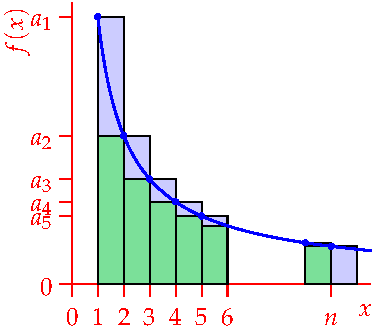
\includegraphics[scale=0.95]{integraltest}
\end{thm}

\begin{proof}
	We need only interpret the picture as describing upper and lower Riemann sums:
	\[
		\int_1^{n+1}f(x)\,\dx\le\textcolor{blue}{\sum_{k=1}^n a_k} =s_n= a_1+\textcolor{Green}{\sum_{k=2}^na_k}\le a_1+\int_1^nf(x)\,\dx \tag*{($\ast$)}
	\]
	Take limits as $n\to\infty$ for the result.
\end{proof}


Even for divergent sums, $(\ast)$ allows us to estimate the growth of $(s_n)$. For greater accuracy, we may evaluate the first few terms explicitly and modify the integral test to estimate the remainder.\smallbreak

An important application of the integral test is to provide a complete description of the convergence status of \textbf{$p$-series}: a useful family of series to which others may be compared.

\begin{cor}{$p$-series}{pseries}
 	Let $p>0$. The series $\sum\frac 1{n^p}$ converges if and only if $p>1$.
\end{cor}

\goodbreak


\begin{examples}{}{inttestex}
	\exstart $\smash{\sum\frac 1{n^3}}$ converges (it is a $p$-series with $p>1$). Moreover,
	\[
		\int_1^\infty\frac 1{x^3}\,\dx 
		=\lim_{b\to\infty}\left[-\frac 12x^{-2}\right]_1^b 
		=\frac 12 
		\implies \frac 12\le \sum_{n=1}^\infty\frac 1{n^3}\le\frac 32
	\]
	This is a poor estimate, particularly the lower bound. For a quick improvement, evaluate the first term and re-run the test starting at $n=2$:
	\[
		1+\int_{2}^\infty\frac 1{x^3}\,\dx 
		\le\sum_{n=1}^\infty \frac 1{n^3} 
		\le 1+\frac 18 +\int_{2}^\infty\frac 1{x^3}\,\dx
		\implies 1+\frac 18\le \sum_{n=1}^\infty \frac 1{n^3}\le 1+\frac 14
	\]
	If greater accuracy is required, more terms can be explicitly evaluated.
	
	\goodbreak
	
	\begin{enumerate}\setcounter{enumi}{1}	
	% 	\item The function $f(x)=x^{-2}\sin(x^{-1})$ is positive and decreasing. Moreover, with the substitution $u=x^{-1}$, we have a convergent integral:
	% 	\[\int_1^\infty f(x)\,\dx =\int_0^1 \sin u\,\du=1-\cos(1)\]
	% 	It follows that the series $\displaystyle \sum_{n=1}^\infty \frac 1{n^2}\sin\left(\frac 1n\right)$ converges. Of course this is utterly trivial by the comparison test.
		
		\item In Example \ref{ex:harmonic}, we used the Cauchy criterion to show that the harmonic series diverges to $\infty$. The integral test makes this much easier and allows us to estimate how many terms are required for the partial sum to $s_n$ to reach a certain threshold: 10 say. Since
		\[
			\ln(n+1) =\int_1^{n+1}\frac 1x\,\dx
			\le s_n=\sum_{k=1}^n\frac 1k
			\le 1+\int_1^n\frac 1x\,\dx =1+\ln n
		\]
		we see that $s_n\approx 10$ requires
		\[
			\ln(n+1)\le 10 \le 1+\ln n
		 	\implies e^9\le n\le e^{10}-1 \implies 8104\le n\le 22025	
		\]
		The harmonic series diverges to infinity, but it does so \emph{very slowly.}
		
		\item\label{ex:integralsuperslow} The integral test shows that $\sum_{n=2}^\infty \frac 1{n\ln n}=\infty$. To exceed 10, somewhere between $10^{3223}$ and $10^{6631}$ terms are required. To exceed 100 requires `roughly' $10^{6\times 10^{42}}$ terms: 1 followed by 1000 zeros for each water molecule in Lake Tahoe puts you at least in the right ballpark\ldots
		
		\item The series $\sum \frac{2n+1}{\sqrt{4n^3-1}}$ diverges to $\infty$ by comparison with the $p$-series $\sum \frac 1{\sqrt n}$.
	\end{enumerate}
\end{examples}



\begin{minipage}[t]{0.6\linewidth}\vspace{0pt}
	\boldsubsubsection{Alternating Series and Conditional Convergence}
	
	Our final test is unique in that it can detect \emph{conditional convergence.} The canonical example is the \emph{alternating harmonic series} (Example \ref*{ex:compexs}.\ref{ex:altharmonic1}). With an eye on generalization, we re-index so that the first term is $a_0=1$:
		\begin{align*}
			s&=\sum_{n=0}^\infty\textcolor{Green}{\frac{(-1)^{n}}{n+1}} =1-\frac 12+\frac 13-\frac 14+\cdots\\
			&=\sum_{n=0}^\infty\textcolor{Green}{(-1)^{n}a_n} =a_0-a_1+a_2-a_3+\cdots
		\end{align*}
\end{minipage}
\hfill
\begin{minipage}[t]{0.39\linewidth}\vspace{5pt}
	\flushright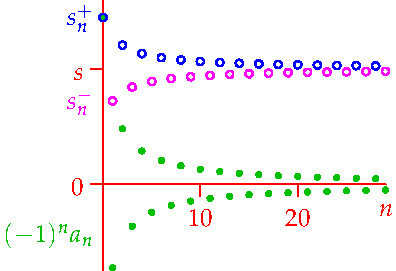
\includegraphics[scale=0.95]{alternatingharmonic}
\end{minipage}
\medbreak

The \emph{alternating} $\pm$-signs give the series its name. Consider the behavior of the sequence of partial sums $(s_n)$, in particular two subsequences $(\textcolor{blue}{s_n^+})=(s_{2n})$ and $(\textcolor{magenta}{s_n^-})=(s_{2n-1})$:
\begin{gather*}
	\textcolor{blue}{s_n^+}=\sum_{k=0}^{2n}(-1)^ka_k 
		 =1 
		 -\biggl(\underbrace{\frac 12-\frac 13}_{a_1-a_2}\biggr) 
		 -\biggl(\underbrace{\frac 12-\frac 13}_{a_3-a_4}\biggr)
		 -\cdots 
		 -\biggl(\underbrace{\frac 1{2n}-\frac 1{2n+1}}_{a_{2n-1}-a_{2n}}\biggr) 
		 \tag{$n\ge 0$}\\
	\textcolor{magenta}{s_n^-}=\sum_{k=0}^{2n-1}(-1)^ka_k 
		=\biggl(\underbrace{1-\frac 12}_{a_0-a_1}\biggr) 
		+\biggl(\underbrace{\frac 13-\frac 14}_{a_2-a_3}\biggr) 
		+\cdots 
		+\biggl(\underbrace{\frac 1{2n-1}-\frac 1{2n}}_{a_{2n-2}-a_{2n-1}}\biggr) 
		\tag{$n\ge 1$}
\end{gather*}
Each bracketed term is non-negative, so $(s_n^+)$ is \textcolor{blue}{monotone-down} and $(s_n^-)$ \textcolor{magenta}{monotone-up.} Moreover,
\[
	\frac 12=\textcolor{magenta}{s_1^-}
	\le \textcolor{magenta}{s_n^-}
	\le \textcolor{magenta}{s_n^-}+a_{2n} 
	= \textcolor{blue}{s_n^+} 
	\le \textcolor{blue}{s_0^+} 
	=1 \tag{$\dag$}
\]
from which both subsequences are \emph{bounded} and thus \emph{convergent.} Not only this, but
\[
	\lim\bigl(\textcolor{blue}{s_n^+} 
	-\textcolor{magenta}{s_n^-}\bigr) 
	=\lim a_{2n} =0
\]
shows that the limits of both subsequences are \emph{identical} (of course both are $s$).

\goodbreak

The above discussion depends only on \textcolor{blue}{two simple properties} of the sequence $(a_n)$. We've therefore proved a general statement.

\begin{thm}{Alternating series test}{}
	Suppose $(a_n)$ is \textcolor{blue}{monotone-down} and that $\textcolor{blue}{\lim a_n=0}$. Then:
	\begin{enumerate}
	  \item The alternating series $s=\sum (-1)^na_n$ converges.
		\item If $(s_n)$ is the sequence of partial sums, then $\nm{s-s_n}\le a_{n+1}$.
	\end{enumerate} 
\end{thm}

Think about where the \textcolor{blue}{hypotheses} regarding $(a_n)$ are used in the proof.\smallbreak

It can be shown that the alternating harmonic series converges to $\ln 2$, though the estimates provided by the alternating series test are very poor: to guarantee accuracy to two decimal place requires us to sum 100 terms of the series!

\begin{examples}{}{}
	\exstart Since $a_n=\frac 1{n!}$ converges monotone-down to zero, the alternating series $\sum\frac{(-1)^n}{n!}$ converges. By evaluating $s_8$ and $s_9$ explicitly, we see that
	\[
		0.3678791887\ldots
		\le\sum_{n=0}^\infty\frac{(-1)^n}{n!}
		\le 0.3678819444\ldots
	\]
	yielding an estimate of $0.36788$ to 5 decimal places (the exact value is in fact $e^{-1}$). The alternating series test is only needed for the estimate, since the series converges absolutely.
	
	\begin{enumerate}\setcounter{enumi}{1}
	  \item The series $\sum_{n=2}^\infty\frac{\sin\frac\pi 2n}{\ln n}$ can be viewed as an alternating series since every \emph{even} term is zero. Writing $m=2n+1$, we obtain
	  \[
	  	\sum_{n=2}^\infty\frac{\sin\frac\pi 2n}{\ln n} 
	  	=\sum_{m=1}^\infty\frac{\sin(\pi m+\frac\pi 2)}{\ln(2m+1)}
	  	=\sum_{m=1}^\infty\frac{(-1)^{m}}{\ln(2m+1)} 
	  \]
	  Since $\frac 1{\ln(2m+1)}$ decreases to zero, the alternating series test demonstrates convergence.
	\end{enumerate}
\end{examples}

\smallskip

\boldsubsubsection{Rearranging Infinite Series}

A \emph{rearrangement} of an infinite series $\sum a_n$ is a series that results from changing the \emph{order} of the terms of the sequence $(a_n)$ \emph{before} computing the partial sums. The new series must still use every term of the original. Since the new sequence of partials sums is likely different, we shouldn't assume that the rearranged series has the same convergence properties as the old.

\begin{example}{}{riemannrearrangement}
	We rearrange the alternating harmonic series by summing \textcolor{blue}{two positive terms} before each \textcolor{magenta}{negative term}:
	\[	
		\textcolor{blue}{1}+\textcolor{blue}{\frac 13} 
		-\textcolor{magenta}{\frac 12}
		+\textcolor{blue}{\frac 15} +\textcolor{blue}{\frac 17} 
		-\textcolor{magenta}{\frac 14}
		+\textcolor{blue}{\frac 19} +\textcolor{blue}{\frac 1{11}} 
		-\textcolor{magenta}{\frac 16}
		+\cdots 
		+\textcolor{blue}{\frac 1{4n-3}} +\textcolor{blue}{\frac 1{4n-1}} 
		-\textcolor{magenta}{\frac 1{2n}} 
		+\cdots
	\]
	Every term of the original sequence is used here, so this is a genuine rearrangement. It is perhaps surprising to discover that the new series converges, though its limit is \emph{not the same} as the original alternating harmonic series! We leave the details to Exercise \ref{exs:riemannrearrangement}. This behavior is quite different to that of finite sums, where the order of summation makes no difference at all. 
\end{example}

\goodbreak

The general situation is summarized in a famous result of Riemann. The first part says that absolutely convergent series behave just like finite sums. Conditionally convergent series are much stranger.\footnotemark{}

\begin{thm}{Riemann rearrangement}{}
	\exstart If a series converges absolutely, then all rearrangements converge to the same limit.
	\begin{enumerate}\setcounter{enumi}{1}
	  \item If a series converges conditionally and $s\in\R\cup\{\pm\infty\}$ is given, then there exists a rearrangement which tends to $s$.
% 	  \item If $\sum a_n$ converges conditionally and $s^+\ge s^-$ (both in $\R\cup\{\pm\infty\}$) are given, then there exists a rearrangement whose sequence of partial sums satisfies $\limsup s_n=s^+$ and $\liminf s_n=s^-$.
	\end{enumerate}
\end{thm}

\footnotetext{%
 	Riemann's second result is in fact even stronger. Conditionally convergent series also have rearrangements whose sequence of partial sums diverges by oscillation to any given $\liminf s_n<\limsup s_n$!%
}

We omit the proofs since they are prohibitively lengthy. Instead we illustrate the rough idea of part 2 via an example.

\begin{example}{}{riemannrearrange}
	We show how to construct a rearrangement of the alternating harmonic series which converges to $s=\sqrt 2=1.41421\ldots$\smallbreak
	First we convince ourselves that the sum of the positive terms $\sum a_n^+$ diverges to infinity. The comparison test makes this easy:
	\[
		\frac 1{2n-1}>\frac 1{2n}\implies \sum a_n^+=\sum \frac 1{2n-1}>\frac 12\sum \frac 1n=\infty
	\]
	The negative terms also diverge: $\sum a_n^-=-\infty$. Construction of the rearrangement is inductive.
	\begin{enumerate}
	  \item Sum just enough positive terms $S_1 =a_1^++a_2^++\cdots+a_{n_1}^+$ \emph{in order} until the partial sum exceeds $s$: plainly $S_1 =\textcolor{blue}{1}+\textcolor{blue}{\frac 13}+\textcolor{blue}{\frac 15} \approx 1.53333$ will do here.
		\item Add negative terms starting at the beginning of the sequence until the sum is less than $s$:
		\[
			S_2=S_1+(a_1^-+a_2^-+\cdots+a_{m_1}^-)
			=\textcolor{blue}{1}+\textcolor{blue}{\frac 13}+\textcolor{blue}{\frac 15} -\textcolor{magenta}{\frac 12} = 1.0333\cdots<s
		\]
		\item Repeat: add positive terms until the sum just exceeds $s$, then add negative terms, etc.,
		\begin{gather*}
			S_3=S_2 +\textcolor{blue}{\frac 17} +\textcolor{blue}{\frac 19} 
			+\textcolor{blue}{\frac 1{11}} +\textcolor{blue}{\frac 1{13}} 
			=1.4551\ldots>s,\qquad 
			S_4=S_3 -\textcolor{magenta}{\frac 14} =1.2051\ldots<s
		\end{gather*}
	\end{enumerate}
	Continuing the process ad infinitum, we claim that	
	\[
		s =\sqrt 2=
		\textcolor{blue}{1} +\textcolor{blue}{\frac 13}
		+\textcolor{blue}{\frac 15} -\textcolor{magenta}{\frac 12} 
		+\textcolor{blue}{\frac 17} +\textcolor{blue}{\frac 19} 
		+\textcolor{blue}{\frac 1{11}} +\textcolor{blue}{\frac 1{13}} 
		-\textcolor{magenta}{\frac 14} +\textcolor{blue}{\frac 1{15}}
		+\textcolor{blue}{\frac 1{17}} +\textcolor{blue}{\frac 1{19}}
		+\textcolor{blue}{\frac 1{21}} -\textcolor{magenta}{\frac 16}
		+\textcolor{blue}{\frac 1{23}} +\textcolor{blue}{\frac 1{25}}
		+\cdots 
	\]
% 	\[
% 		s=\textcolor{blue}{1}-\textcolor{magenta}{\frac 12}-\textcolor{magenta}{\frac 14} +\textcolor{blue}{\frac 13} -\textcolor{magenta}{\frac 16} -\textcolor{magenta}{\frac 18} +\textcolor{blue}{\frac 15} -\textcolor{magenta}{\frac 1{10}} +\textcolor{blue}{\frac 17}  -\textcolor{magenta}{\frac 1{12}}  -\textcolor{magenta}{\frac 1{14}} +\textcolor{blue}{\frac 19} -\textcolor{magenta}{\frac 1{16}} -\textcolor{magenta}{\frac 1{18}} +\textcolor{blue}{\frac 1{11}}  -\textcolor{magenta}{\frac 1{20}} +\textcolor{blue}{\frac 1{13}} -\cdots 
% 	\]
	To see why, observe:
	\begin{itemize}
	  \item Since $\sum a_n^+=\infty$ and $\sum a_n^-=-\infty$, at each stage we need only add/subtract \emph{finitely many terms.}
	  \item All terms of the original sequence $(a_n)$ are eventually used since we add the positive (negative) terms \emph{in order.} E.g., $a_{495}=\frac 1{495}$ appears, \emph{at the latest,} during the 495\th{} positive-addition phase.
	  \item $\nm{S_n-s}\le \nm{a_{m_n}}$, where $a_{m_n}$ is the final term used at the $n\th$ stage. The right hand side converges to zero ($n\th$-term test!), whence $\lim S_n=s$. 
	\end{itemize}
\end{example}


\begin{exercises}{}{}
	\emph{Key concepts:\quad Integral test and approximation,\quad Alternating series and approximation}

	\begin{enumerate}  
		\item%[4.] and others
		 Use the integral test to determine whether the series $\sum_{n=1}^\infty\frac 1{n^2+1}$ converges or diverges.
	
	  \item Prove Corollary \ref{cor:pseries} regarding the convergence/divergence of $p$-series.
	  
	  
	  \item Let $\smash{s_n=\sum_{k=1}^n\frac 1{\sqrt k}}$. Estimate how many terms are required before $s_n\ge 100$.
	
	
		\item (Example \ref*{ex:inttestex}.\ref{ex:integralsuperslow})\lstsp Verify the claim that $\smash{\sum_{n=2}^\infty\frac 1{n\ln n}=\infty}$ and the claim regarding the estimate.
	%    \item Determine whether $\sum \frac 1{n\ln n\ln\ln n}$ converges or diverges.
	
	  
  \item\begin{enumerate}
    \item Use calculus to show that $a_n=\frac{\ln n}{n^2}$ is monotone-down whenever $n\ge 2$.
    \item Show that $\lim a_n=0$, and that the hypotheses of the integral test are therefore satisfied.%\par
    %(\emph{Hint: You may use without proof that $\ln n<n$ for large $n$})
    \item Determine whether the series $\sum_{n=2}^\infty\frac{\ln n}{n^2}$ converges or diverges.
  \end{enumerate}

	  
	\item\begin{enumerate}
	  \item %[6a]
	  Give an example of a series $\sum a_n$ which converges, but for which $\sum a_n^2$ diverges.\par
		(\emph{Exercise \ref*{sec:series}.\ref{exs:seriesmult} really requires that $\sum a_n$ be absolutely convergent!})
		\item Give an example of a divergent series $\sum b_n$ for which $\sum b_n^2$ converges.
	 \end{enumerate}
	  
	  
	 \item Suppose $(a_n)$ satisfies the hypotheses of the alternating series test except that $\lim a_n=a$  is \textbf{strictly positive}. What can you say about the sequences $(s_n^+)$ and $(s_n^-)$ and the series $\sum (-1)^na_n$?
	  
	  
	 \item\label{exs:integralestimates}
	Let $a_n=\frac 1n$ have partial sum $s_n=\sum_{k=1}^na_n$, and define a new sequence $(t_n)$ by
	\[
		t_n=s_n-\ln n =\smash{1+\frac 12+\cdots +\frac 1n-\ln n}
	\]
	Prove that $(t_n)$ is a positive, monotone-down sequence, which therefore converges.\footnotemark{}\par
	(\emph{Hint: You'll need the mean value theorem from elementary calculus})
	
		
	\item Suppose $\sum a_n$ is conditionally convergent and let $\sum a_n^+$ be the series obtained by summing, in order, the \emph{positive} terms of the sequence $(a_n)$. Prove that $\sum a_n^+=\infty$.
	
		
	\item\begin{enumerate}
	  \item Show that the series $\sum_{n=1}^\infty \frac{(-1)^nn}{n^2+1}$ is conditionally convergent to some real number $s$.
	  \item How many terms are required for the partial sum $s_n$ to approximate $s$ to within $0.01$.
	  \item Following Example \ref{ex:riemannrearrange}, use a calculator to state the first twelve terms in a rearrangement of the series in part (a) which converges to 0. 
	\end{enumerate} 
		
		
	\item\label{exs:riemannrearrangement} Recall the rearrangement of the alternating harmonic series in Example \ref{ex:riemannrearrangement}.
	\begin{enumerate}
		\item Verify that the \emph{subsequence} of partial sums $(s_{3n})$ is monotone-up, by checking that
		\[
			b_n:=\frac 1{4n-3}+\frac 1{4n-1}-\frac 1{2n}>0,\quad\text{ for all $n\in\N$}
		\]
		\item Use the comparison test to show that $\sum b_n$ converges.
		\item Prove that the rearranged series converges to some value $s>\frac 56$.\par
		(\emph{Thus $s>\ln 2\approx 0.69$, the limit of the original alternating harmonic series})
		\end{enumerate}
			
	\end{enumerate}
\end{exercises}

\vspace{-15pt}

\footnotetext{%
	The limit $\gamma:=\lim t_n\approx 0.5772$ is the \emph{Euler--Mascheroni constant.} It appears in several mathematical identities, and yet very little about it is understood; it is not even known whether $\gamma$ is irrational!%
}